\documentclass[12pt]{article}
\usepackage[utf8]{inputenc}
\usepackage{amsmath}
\usepackage{mathrsfs}
\usepackage{amssymb}
\usepackage{amsfonts}

\DeclareMathOperator{\logit}{logit}
\DeclareMathOperator*{\argmax}{arg\,max}
\DeclareMathOperator*{\argmin}{arg\,min}

\usepackage[
    a4paper,
    left = 2.5cm,
    right = 2.5cm,
    top = 2.5cm,
    bottom = 2.5cm
]{geometry}

\usepackage{graphicx}
\usepackage[headings]{fullpage}
\usepackage{xcolor}
\usepackage{hyperref}
\usepackage{fancyhdr}
 %For aligned formulas
 \usepackage{IEEEtrantools}
\usepackage{listings} %Source code listings https://en.wikibooks.org/wiki/LaTeX/Source_Code_Listings

% \lstset{
%     language=R, %You can always set to another language
%     breaklines,
%     deletekeywords={category},
%     basicstyle=\ttfamily\footnotesize,
%     otherkeywords={!,!=,~,\$,*,\&,\%/\%,\%*\%,\%\%,<-,<<-},
%     literate={~}{$\sim$}1 {<-}{{$\gets$}}1
% }

\usepackage[
    backend=biber,
    style=apa,
    maxcitenames=2,
    mincitenames=1,
    sorting=ynt
    ]{biblatex}
\addbibresource{bibfile.bib}

\setlength{\headheight}{15pt}
\pagestyle{fancy}
\fancyhf{}
\rhead{Odole, Cunha, and Murthy} % Fill in your name
%\lhead{Bayesian Statistics \& Probabilistic Machine Learning---Project Report}
\rfoot{Page \thepage}


\begin{document}

\begin{titlepage}
        \centering % Center all text
        \vspace*{\baselineskip} % White space at the top of the page
        
        {\huge YOUR TITLE}\\[0.2\baselineskip] % Title
        
        
        \vspace*{\baselineskip}
        
        {\Large --- Project Report ---\\
          Advanced Bayesian Data Analysis\\[\baselineskip]} % Tagline(s) or further description
        \vspace*{\baselineskip}
        
        {\LARGE Eldaleona Odole,  Leonor Cunha, and Anarghya Murthy\\[\baselineskip]} % Editor list  
        
        \vspace*{\baselineskip}

        \vfill
        
        \today \par % Location and year
        
        \vspace*{\baselineskip}

        {\itshape TU Dortmund University\par} % Editor affiliation
    \end{titlepage}

\clearpage

% \section{Template}
% This is a template for the project report in the course Advanced Bayesian Data Analysis.
% Fill in your title and names for the title page and header and follow the general structure. You don't have to use multiple chapters or sections at all for this short report, but if you do, don't go further than subsections--- \textcite{feynman1963lnphysics} didn't need to\ldots

% Some examples on how to use \LaTeX{} are shown below. If you want to reference something, you can do it as so:
% \textcite{mcelreath2016statistical}.

% \subsection{Images}
% \begin{figure}
%     \begin{center}
%     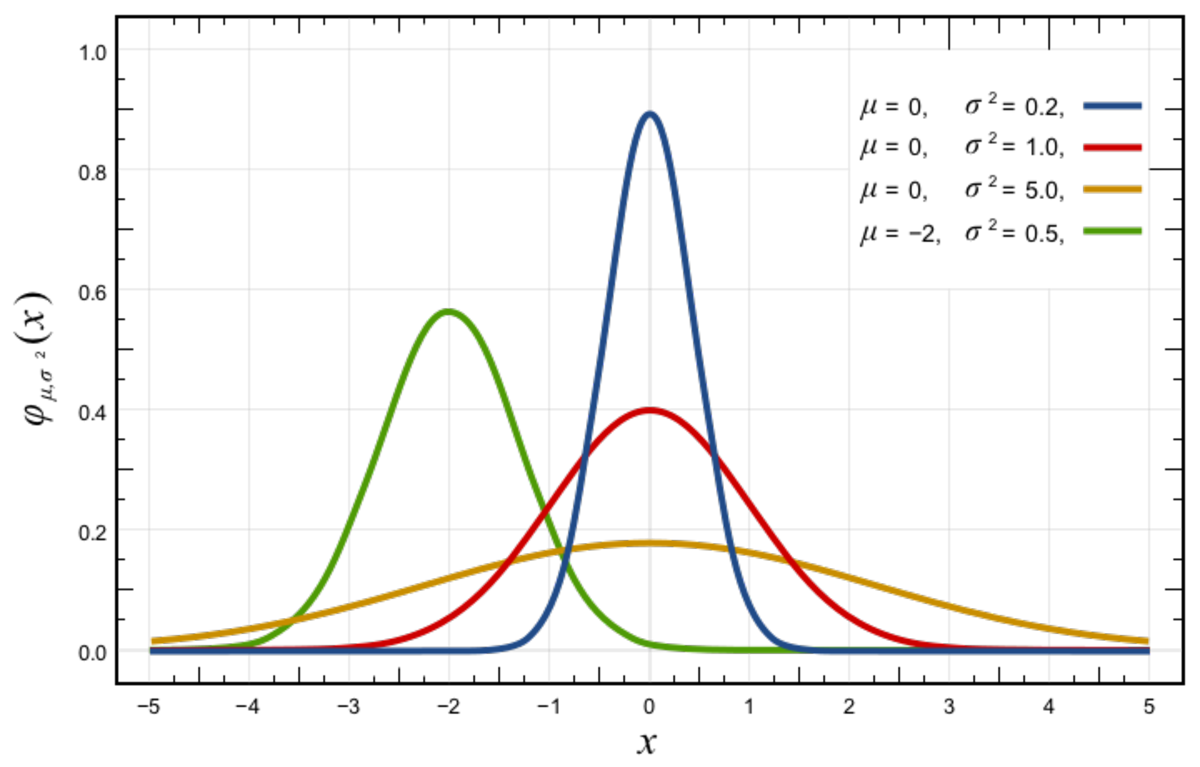
\includegraphics[width=0.5\textwidth]{figures/Normal_Distribution_PDF.pdf} %try to never force a figure placement
%     \caption{Probability density function for the Normal distribution. The red curve is the standard normal distribution. [By Inductiveload - self-made, Mathematica, Inkscape, Public Domain, \url{https://commons.wikimedia.org/w/index.php?curid=3817954}]}
%     \label{fig:normal_sample}
%     \end{center}
% \end{figure}

% This is an example for how to insert images into your document. When talking about a figure, you should always point out which one you mean, i.e., ``As you can see in Figure~\ref{fig:normal_sample}.''

% \subsection{Tables}
% A table has a caption \textit{above} the table as in Table~\ref{tab:my_label}.

% \begin{table} %You can place [h] immediately after \begin{table} to force the placement of the table. Generally speaking never do that---LaTeX usually places them in a sane way!
%     \centering
%     \caption{My caption.}
%     \label{tab:my_label}
%     \begin{tabular}{c|l} % l, r, and c justified inside cells.
%         \hline
%          Poisson & $\lambda$ \\ % Always end a line with \\
%          Normal &  $\mu$ and $\sigma$\\ 
%         \hline
%     \end{tabular}
% \end{table}

% \subsection{Formulas}
% This is a small example for how to include formulas into your document. $a^2 + b^2 = c^2$ will inline a formula, while
% $$c \leq a + b$$
% will give the formula its own line.

% \subsection{Formulas}
% You also might want to write out models:

% {\footnotesize % you align formulas using & 
% \begin{IEEEeqnarray*}{rCl}
% \mathrm{L}_i & \sim & \mathrm{Binomial}(n_i,p_i)\\
% \mathrm{logit}(p_i) & = & \alpha_{\mathrm{SUBJECT}[i]} + (\beta_P + \beta_{PC}C_i)P_i\\
% \alpha_{\mathrm{SUBJECT}} & \sim & \mathrm{Normal}(0,10) \\
% \beta_P & \sim & \mathrm{Normal}(0,10)\\
% \beta_{PC} & \sim & \mathrm{Normal}(0,10)
% \end{IEEEeqnarray*}
% }


% \subsection{Source code}
% Of course, formatting source code is always nice.
% \begin{lstlisting}
% m <- map(
%     alist(
%         height ~ dnorm(mu, sigma),
%         mu <- a + b*weight,
%         a ~ dnorm(0, 100),
%         b ~ dnorm(0, 10),
%         sigma ~ dunif(0, 50) 
%     ), 
%     data=d2)
% \end{lstlisting}

% \subsection{Math fonts}
% Different math fonts are also available to you:

% $\mathrm{ABCDE abcde 1234}$

% $\mathit{ABCDE abcde 1234}$

% $\mathnormal{ABCDEabcde1234}$

% $\mathcal{ABCDE abcde 1234}$

% $\mathscr{ABCDE abcde 1234}$

% $\mathfrak{ABCDE abcde 1234}$

% $\mathbb{ABCDE abcde 1234}$

\section{Introduction}


\textcolor{red}{notes to ourselves about things that should go in each section can be in red like this so we dont forget to delete them :)}

Every two years the United States elects 435 officials to the House of Representatives. The 435 House seats are allocated roughly proportional to population with additional constraint that each state must have at least one seat in the House of Representatives. However, despite being roughly equivalent in population size, the characteristics of voters living in each district varies greatly by district.

Although technically a multiparty system, the U.S. is often called a two party system due to the domination of Democrats and Republicans at all levels of govenrment (cite). These parties dominate because political candidates are only required to get a plurality of votes, of which the two largest parties often reach. Additionaly would be third-party voters, will often vote for one of the two major parties so ensure their voice is heard, rather than using thier vote on a candidate who will likely not win (cite). Within our dataset, there are no districts represented by a third-party candidate and as such we often refer to the U.S. as being a two party system.  The association between a voters demographics (gender, age, education etc.) and their propensity to vote for either a democratic or republican candidates is a topic of extensive study. However, little is known about the relationship between voting outcomes and the voters environment.  In a very general sense, conventional wisdom says that cities tend to be more “blue”, meaning voters in large cities tend to vote for democrats. Our project is focused on characterizing this relationship more concretely.

To answer our question about the nature of the relationship between urbanizaiton and partisan voting outcomes, we choose to investigate the 2022 House Election. This election takes places during a non-presidential year, which may cause additonal effects, this election also takes place most recently after the 2020 Census, allowing us to use the most recently available demographic data.

Within this report we combine demographic data and urbanization data into a logistic regression model to predict the district voting outcomes of the 2022 House Election. The parameters 
% Previous attempts? 


\section{Dataset}


Our dataset was made by combining three independent datasets related to the 2022 House election. The first dataset is the publically available urbanization dataset published by fivethirty eight from which we incorporate the variables urbanization index  and (urban) grouping into our final dataset \cite{urbanizationdataset}. From the description of the dataset: "The urbanization index is calculated as the natural logarithm of the average number of people living within a five-mile radius of every census tract in a given district, based on a weighted average of the population of each census tract. The population of a census tract is according to 2020 census data. This provides a numerical value for how urban or rural a district is. " \cite{urbanizationdataset}. The urbanization dataset was put together by FiveThirtyEight as part of their analysis  \textit{The Republican Path To a House Majority Goes Through The Suburbs} which gave election predictions leading up to the 2022 U.S. Congressional Eleciton \cite{538urbanizationarticle}. 
% maybe add something about this analysis? 

The second dataset used in our analysis the Election Results Dataset from FiveThirtyEight \cite{electionresultsdataset}. It is a continuously updated repository of United States Govenor, Congressional and Presidential elections. As this dataset includes all elections going back to 1998, we only used a subset of the data relevant to the 2022 House Election. From this dataset we used the party, state, and winner variables. 

The third data used in our analysis is a subset of the 2022 American Commuity Survey Data. The American Community Survey is a yearly survey collecting information about the occupations, education attainment, income and other demographic information carried out by the United States Census Bureau. The United States Census Bureau provides an online tool to access its extensive survey database, which can then be filtered and refined for further analysis. For our analysis we used the following variables for each House district; 



\subsection{Data Cleaning}

In the initial cleaning we wanted all the variable to be on roughly the same scale to aid in convergence times. In order to do that we roughly scaled median income and total population by dividing total population by one million and dividing median income by one hundred thousand. This brought each of these to roughly the same scale as the other variables that are in the range of zero to one as they are percentages. 

\section{Models}

To describe our approach we wanted to test different models that incorporate the geographical hierarchy into the model. We made several common assumptions for the the four models that we compared with addtional more specific assumptions for each model. The first common assumption we made was that district voting outcomes can be modeled via logistic regression. This assumption gets at the basic logic of our models. As we said previously the outcomes of any particular district electoral race is binary (democrat/republic) so it is most appropriate to choose a modeling technique that can model binary outcomes. 

\textit{Why did we choose logisitic regression?}

We then moved on to our assumptions about the parameters of the linear regression model within the logistic regression model. We also assume that geography is a characteristic of each district that can be modeled hierarchical. For that reason we assume that each district is exchangeable within each state and that each state is exchangeable within each region. We assume this because for complicated historical reasons certain regiions of the united states are more similar to eachother than others. For example the Southern United states tends to be more religious and religous people tend to vote more conservatively, as a result the parameter associated with region would likely be smaller or more negative as compared to other regions. 
We also are assuming that in some regions the value of urban index is more informative than others, the logic being that a city in a rural area will likely have stronger signal than an city among a bunch of other cities. 

We also 


\subsubsection*{Model 1}

Let the response variable 'Winning Party' be \(y\), and \(i\), \(j\), and \(k\) be the indices for the district, state, and region respectively. 

\[y_{i,j,k} \sim Ber.(logit^{-1}(\theta_{j}))\]


\begin{equation}
	\begin{aligned}
		\theta_{j,k} = &\beta_0 + \beta_1 \cdot \text{Pct\_Women} + \beta_2 \cdot \text{Urban\_Index} + \beta_{2,j} \cdot \text{Urban\_Index} \\
		&+ \beta_3 \cdot \text{Pct\_Bachelor's} + \beta_{3,k} \cdot \text{Pct\_Bach.} + \beta_{4} \cdot \text{Median\_Income} \\ 
		&+ \beta_{4,j} \cdot \text{Median\_Income} + \beta_{5} \cdot \text{Pct\_Retirees}
	\end{aligned}
\end{equation}










\section{Priors}

\textcolor{red}{A table summarizing priors for each model would be nice here}


%% Priors
%\[\beta_0 \sim \text{Normal}(0, 0.5)\]
%\[\beta_1, \beta_2 \sim \text{Normal}(0, 1); \beta_3 \sim \text{Cauchy(0,1)}\] 
%\[\beta_4 \sim \text{Normal}(0,1); \beta_5 \sim \text{t}(1,-1,1)\]
%
%
%\[\beta_{2,j} \sim \text{Normal}(0, \sigma_{\beta_{2,j}})\]
%
%\[\beta_{3,k} \sim \text{Normal}(0, \sigma_{\beta_{3,k}})\]
%
%\[\beta_{4,j} \sim \text{Normal}(0, \sigma_{\beta_{4,j}})\]
%
%\[\sigma_{\beta_{2,j}} \sim \text{Gamma}(2,5) \]
%
%\[\sigma_{\beta_{3,k}} \sim \text{Normal}(0,1) \]
%
%\[\sigma_{\beta_{4,j}} \sim \text{Normal}(0,1) \]




For many of our parameters we picked Normal distributions [reasons]

For the intercept $\beta_0$ in Model 1 we set a Normal prior centered at zero with a small standard deviation. This represents our assumption that the probability of either party winning is roughly 50\% (corresponding to a $\theta_{j,k}$ of zero) when all other factors are absent. [wrong]



In Model 1, neither Pct.Women nor Pct.Retirees are modeled hierarchically. 


The percentage of women is roughly the same in every district, so we do not expect this covariate to have a strong effect on the probability of either party winning, i.e, we expect $\beta_{women}$ to be close to zero. So, we set a prior for this slope which is centered around zero and has little variability: a standard normal prior. 

The Percentage of retirees in each district negatively correlates with the probability of a Democrat winning, but we do not know how strong this effect ought to be. Therefore, for the prior on $\beta_{Pct.Retirees}$ we chose a distribution centered around a negative number, and with relatively heavy tails, reflecting our uncertainty. 



The effects of urban index, percentage of bachelor degrees, and median income are all parameterized in 2 hierarchical levels: an average slope across all districts, and a varying slope by group (State or Region), $\beta_{covariate,j}$ or $\beta_{covariate,k}$, which follows a Normal distribution centered at zero with standard deviation modeled at group level (by a hyperprior).

 
For the average component of the urbanindex slope we opted for a standard normal prior. We chose not to make assumptions on the sign of the effect of this variable, as it is this variable that we are interested in studying. So, we set comparatively less-informative priors on the parameters representing the effect of the index.


As we expected the average effects of both Median Income and Pct Bscs to be positive in some cases and negative in others, we picked symmetric priors for both $\beta_{Pct.Bsc}$ and $\beta_{Med.Income}$. We are, however, less sure about the average null effect of the Percentage of Bachelor degrees, so for this slope parameter we opted for a prior with 'fatter tails', the standard Cauchy distribution rather than the Normal one.


For the hyperparameters, we chose a half standard normal prior for both the standard deviations of $\beta_{Pct.Bsc,k}$ and $\beta_{Med.Income,j}$. This is a narrow distribution, with most values falling between 0 and 1, as we expect to see weak effects for these covariates, and thus small standard deviations (and positive, as any SD is by definition). For the standard deviation of $\beta_{urbanindex,j}$, on the contrary, we opted for a less informative prior. Again, we do not want to make such strong assumptions about the effect of our variable of interest, hence we "allow the estimates to fluctuate more".






\section{Code}


\section{Results}

\textcolor{red}{This section is not on the instructions but is probably the easiest way to talk about the results we got }




\section{Convergence Diagnostics}



\section{Model Comparison}


Our four models were built based on somewhat different assumptions about the structure of our data, and all produced slightly different results. We need to know which of these is \textit{better}, that is, which results are more trustworthy and allow us to answer our original research question.
To this end, we measured and compared our models' predictive performance first by looking at absolute predictive performance, then at relative and finally at the Leave-One-Out statistics to compare out-of-sample Predictive Performance.


To measure absolute predictive performance we used the Root Mean of Squared Error (RMSE)
\textcolor{red}{(FORMULA???)}.
This measure works in a similar way to the R squared statistic that is commonly used to assess the fit of linear models, by evaluating differences between observations and model predictions, but RMSE retains the scale of the response variable, meaning it has a direct interpretation in the context of our problem.
It takes into account the uncertainty of the posterior distribution by...


[plots of RMSE draws, overlap for comparison]

[interpretation]



To assess relative predictive performance, we looked at log-likelihood scores, that is, the average of posterior draws' log-likelihoods for each observation
\textcolor{red}{(FORMULA???)}. 
This is a relative predictive performance measure in the sense that it does not tell us anything about the model's predictive performance alone, we need to compare it between different models to establish which is better.
 

[plot of ll scores or likelihood differences?, overlap]

[interpretation]

Note: these metrics are in-sample, so is biased towards more complex models 


In-sample predictive performance measures evaluate only model predictions for the same observations which were used to fit the model in the first place, therefore they tend to favor more complex models.
(In our case, the bigger mmodel (Model 1) was indeed the preferred one using both RMSE and LL scores.?????????????????')
Because we are comparing models with different degrees of complexity, it is essential to check also out-of-sample predictive performance metrics. These metrics are computed by splitting the dataset into training data and test data, fitting the model on the former and assessing the likelihood (ELPD) of the observations in the latter, given the model estimates with the training set.
\textcolor{red}{ELPD FORMULA??????????????}

The way we choose to split the data into training/test sets naturally impacts the ELPD. So, we rely on cross-validation: we do multiple different splits and average over the results. Our chosen method was Leave-One-Out cross-validation, which in theory performs as many splits as observations in the dataset, each time leaving one "out" as the test data. In practice, a different posterior is not actually computed this many times, but rather an estimate from the full model posterior using importance sampling (PSIS).

[LOO statistics table]

According to the LOO statistics, model 1 is the preferred one.

[pareto k estimates issue and momnet matching?]


\section{Prior Sensitivity Analysis}

\textcolor{red}{another table with priors here, maybe not all because thats a lot}

One of the most important parts of Bayesian Data Analysis is setting the prior distributions. The choice of priors could greatly affect the final results in a model..  \textcolor{red}{(cite prior sensitivity guys)}
So, we conducted a prior sensitivity analysis, by refitting our model(s) using alternative priors (which also fit our model assumptions) and assessing the impact in our results.

[BRIEFLY explain new priors, graphs comparing them]



\section{Limitations and Improvements}


\section{Conclusion}

\subsection{Reflection on own learnings}

\textcolor{red}{please lets call this subsection something else, this sounds so childish}


\printbibliography

\end{document}
